\documentclass[a4paper,12pt]{ctexart} % 使用 ctexart 文档类，原生支持中文

% ==================== 宏包引入 ====================
\usepackage{geometry}       % 页面边距设置
\usepackage{graphicx}       % 插入图片
\usepackage{float}          % 图片位置强制固定
\usepackage{booktabs}       % 三线表
\usepackage{amsmath}        % 数学公式
\usepackage{listings}       % 代码块
\usepackage{xcolor}         % 颜色支持
\usepackage{hyperref}       % 目录跳转和超链接
\usepackage{caption}        % 图表标题格式
\usepackage{subcaption}
\usepackage{fancyhdr}       % 页眉页脚

% ==================== 页面设置 ====================
\geometry{left=2.5cm, right=2.5cm, top=2.5cm, bottom=2.5cm}

% ==================== 代码高亮设置 ====================
\definecolor{codegreen}{rgb}{0,0.6,0}
\definecolor{codegray}{rgb}{0.5,0.5,0.5}
\definecolor{codepurple}{rgb}{0.58,0,0.82}
\definecolor{backcolour}{rgb}{0.95,0.95,0.92}

\lstdefinestyle{mystyle}{
    backgroundcolor=\color{backcolour},   
    commentstyle=\color{codegreen},
    keywordstyle=\color{magenta},
    numberstyle=\tiny\color{codegray},
    stringstyle=\color{codepurple},
    basicstyle=\ttfamily\footnotesize,
    breakatwhitespace=false,         
    breaklines=true,
    postbreak=\mbox{\textcolor{red}{$\hookrightarrow$}\space},
    captionpos=b,                    
    keepspaces=true,                 
    numbers=left,                    
    numbersep=5pt,                  
    showspaces=false,                
    showstringspaces=false,
    showtabs=false,                  
    tabsize=2,
    columns=flexible
}
\lstset{style=mystyle, language=Python}

% ==================== 超链接设置 ====================
\hypersetup{
    colorlinks=true,
    linkcolor=black,
    urlcolor=blue,
    citecolor=blue
}

% ==================== 文档信息 ====================
\title{\textbf{自然语言处理实验报告}\\ \large 基于大语言模型的中文分词性能评估与优化}
\author{姓名：张宗桪 \\ 学号：2023K8009991013 \\ 专业：人工智能}
\date{\today}

\begin{document}

% --- 封面 ---
\maketitle
\thispagestyle{empty} 
\newpage 

% --- 目录 ---
\pagestyle{plain}
\tableofcontents
\newpage 

% --- 正文设置 ---
\pagestyle{fancy} 
\fancyhf{} 
\fancyhead[R]{NLP第三次作业报告}
\fancyfoot[C]{\thepage} 
\setlength{\parskip}{0.5em} 

% ================= 正文开始 =================

\section{实验概述}
本次实验旨在利用大语言模型（LLM）完成中文分词任务。实验选取了不同参数规模的模型，基于《人民日报》语料及网络爬取的多源语料进行测试，评估其分词性能，并探究模型参数量对性能的影响，最后通过 In-Context Learning (Few-shot) 方法尝试提升模型分词性能。

\subsection{实验环境与模型}
\begin{itemize}
    \item \textbf{API平台}: Gitee AI Serverless API (https://ai.gitee.com/v1)
    \item \textbf{测试模型}: 
    \begin{itemize}
        \item Qwen3-32B (4元/百万token)
        \item Qwen3-8B (免费模型)
        \item DeepSeek-V3 (8元/百万token)
    \end{itemize}
\end{itemize}
\subsection{API调用示例}
以下代码是aigitee 给的API调用模板：
\begin{lstlisting}[language=Python]
from openai import OpenAI

client = OpenAI(
	base_url="https://ai.gitee.com/v1",
	api_key="XXXXXXXXXXXXXXXXXXXXXXXXXXXXXXXXXXXXXXXX",
	default_headers={"X-Failover-Enabled":"true"},
)

response = client.chat.completions.create(
	messages=[
		{
			"role": "system",
			"content": "You are a helpful and harmless assistant. You should think step-by-step."
		},
		{
			"role": "user",
			"content": "Can you please let us know more details about your "
		}
	],
	model="Qwen3-8B",
	stream=True,
	max_tokens=1024,
	temperature=0.7,
	top_p=0.7,
	extra_body={
		"top_k": 50,
	},
	frequency_penalty=1,
)

fullResponse = ""
print("Response:")
# Print streaming response
for chunk in response:
	if len(chunk.choices) == 0:
		continue
	delta = chunk.choices[0].delta
	# If is thinking content, print it in gray
	if hasattr(delta, 'reasoning_content') and delta.reasoning_content:
		fullResponse += delta.reasoning_content
		print(f"\033[90m{delta.reasoning_content}\033[0m", end="", flush=True)
	elif delta.content:
		fullResponse += delta.content
		print(delta.content, end="", flush=True) 
\end{lstlisting}
% --- 任务一 ---
为了添加提示词，以及隐藏API Key等功能，我将上面的代码进行一些修改：
\begin{itemize}
    \item 将API调用封装在函数中，方便批量处理多行文本,以及改变API调用方式，使之读取储存在文本文件中的API Key。
    \item 在函数内添加了系统提示词明确要求模型保持多行格式返回分词结果。
    \item 在主程序中实现了按批次读取输入文件、调用分词函数、写入输出文件的逻辑，避免因为单次token限制导致的处理失败。
\end{itemize}
部分代码如下所示：
\begin{lstlisting}[language=Python]
system_prompt = (
        "You are a high-efficiency Chinese Word Segmentation tool.\n"
        "Task: Segment the provided text into words using spaces.\n"
        "Strict Constraints:\n"
        "1. The input contains multiple lines. You must process ALL lines.\n"
        "2. Output format must strictly match the line count of the input.\n"
        "3. Do NOT merge lines. Do NOT delete lines.\n"
        "4. Only output the segmented text. No header, no footer, no markdown.\n"
        "5. Use single spaces for segmentation."
    )

with open('api.txt', 'r') as f:
    api_key = f.read().strip()
def main():
    with open(OUTPUT_FILE, 'w', encoding='gbk', errors='ignore') as f:
        pass
    if not os.path.exists(INPUT_FILE):     
        return
    lines = []
    
    with open(INPUT_FILE, 'r', encoding='gbk') as f:
        lines = [line.strip() for line in f.readlines() if line.strip()]

    total_lines = len(lines)
    with open(OUTPUT_FILE, 'a', encoding='gbk', errors='ignore') as f_out:
        for i in range(0, total_lines, BATCH_SIZE):

            batch = lines[i : i + BATCH_SIZE]
            segmented_block = process_batch(batch)
            if segmented_block:
                f_out.write(segmented_block + "\n")
            
            print(" 完成")

    print(f"\n结果已保存至 {OUTPUT_FILE}")
\end{lstlisting}
\section{标准语料上的分词性能测试}
\subsection{数据来源与预处理}
利用北京大学标注的《人民日报》1998年1月分词语料，随机抽取50个句子作为测试集。数据预处理包括去除原标注中的词性标记，仅保留分词空格作为 Ground Truth，以及去除空格作为模型输入文本。
\begin{figure}[H]
    \centering
    
    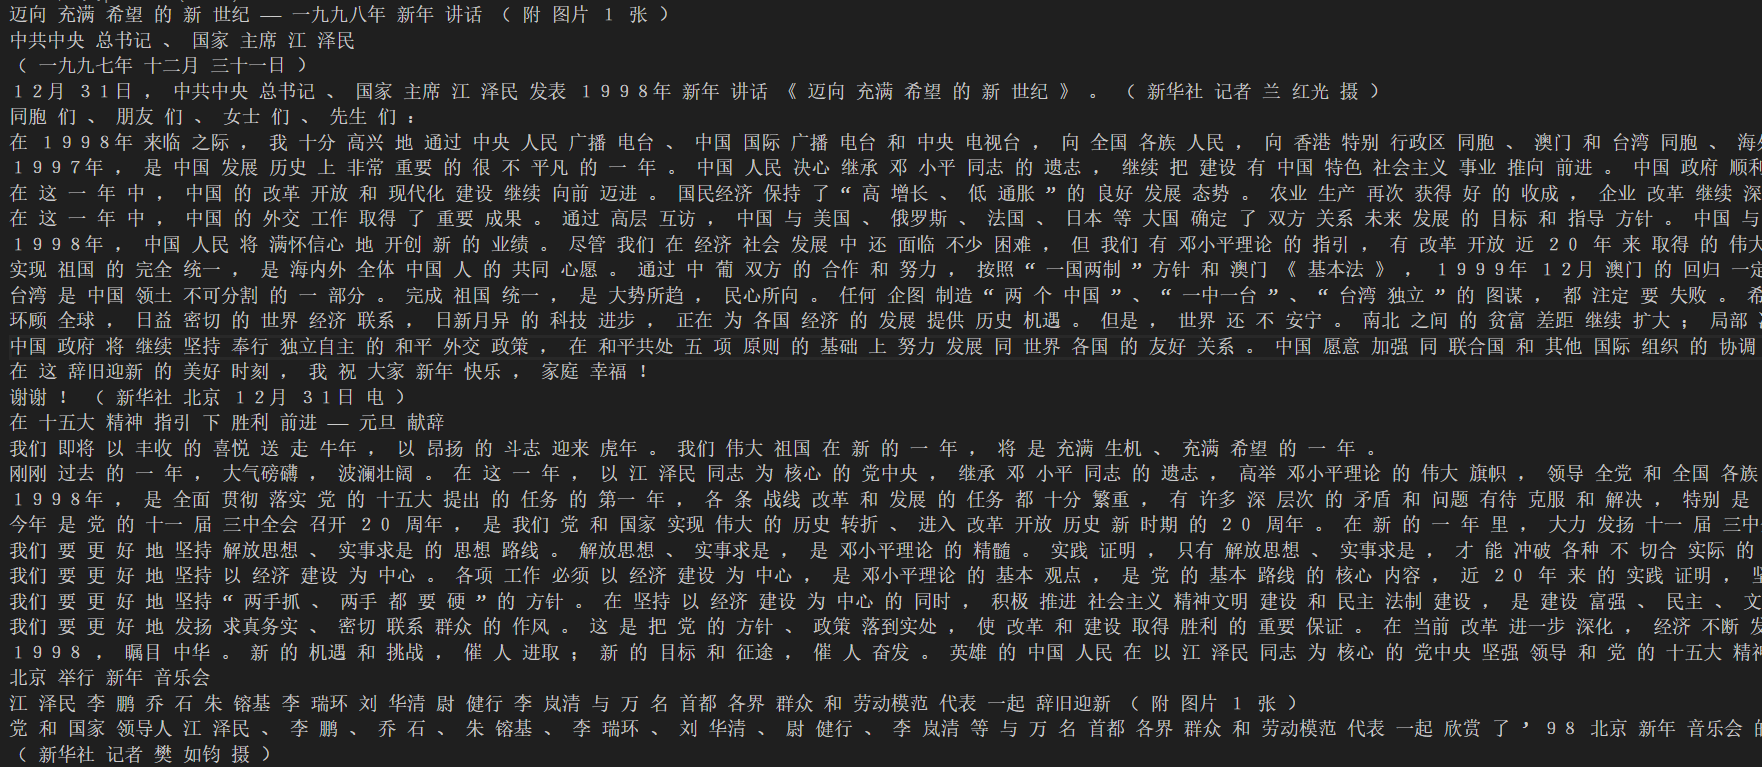
\includegraphics[width=0.8\textwidth]{image/1.png}
    \caption{《人民日报》分词语料示例}
    \label{fig:pku_example}
\end{figure}
\subsection{LLM分词结果}
以下为部分输出示例：
\begin{figure}[H]
    \centering
    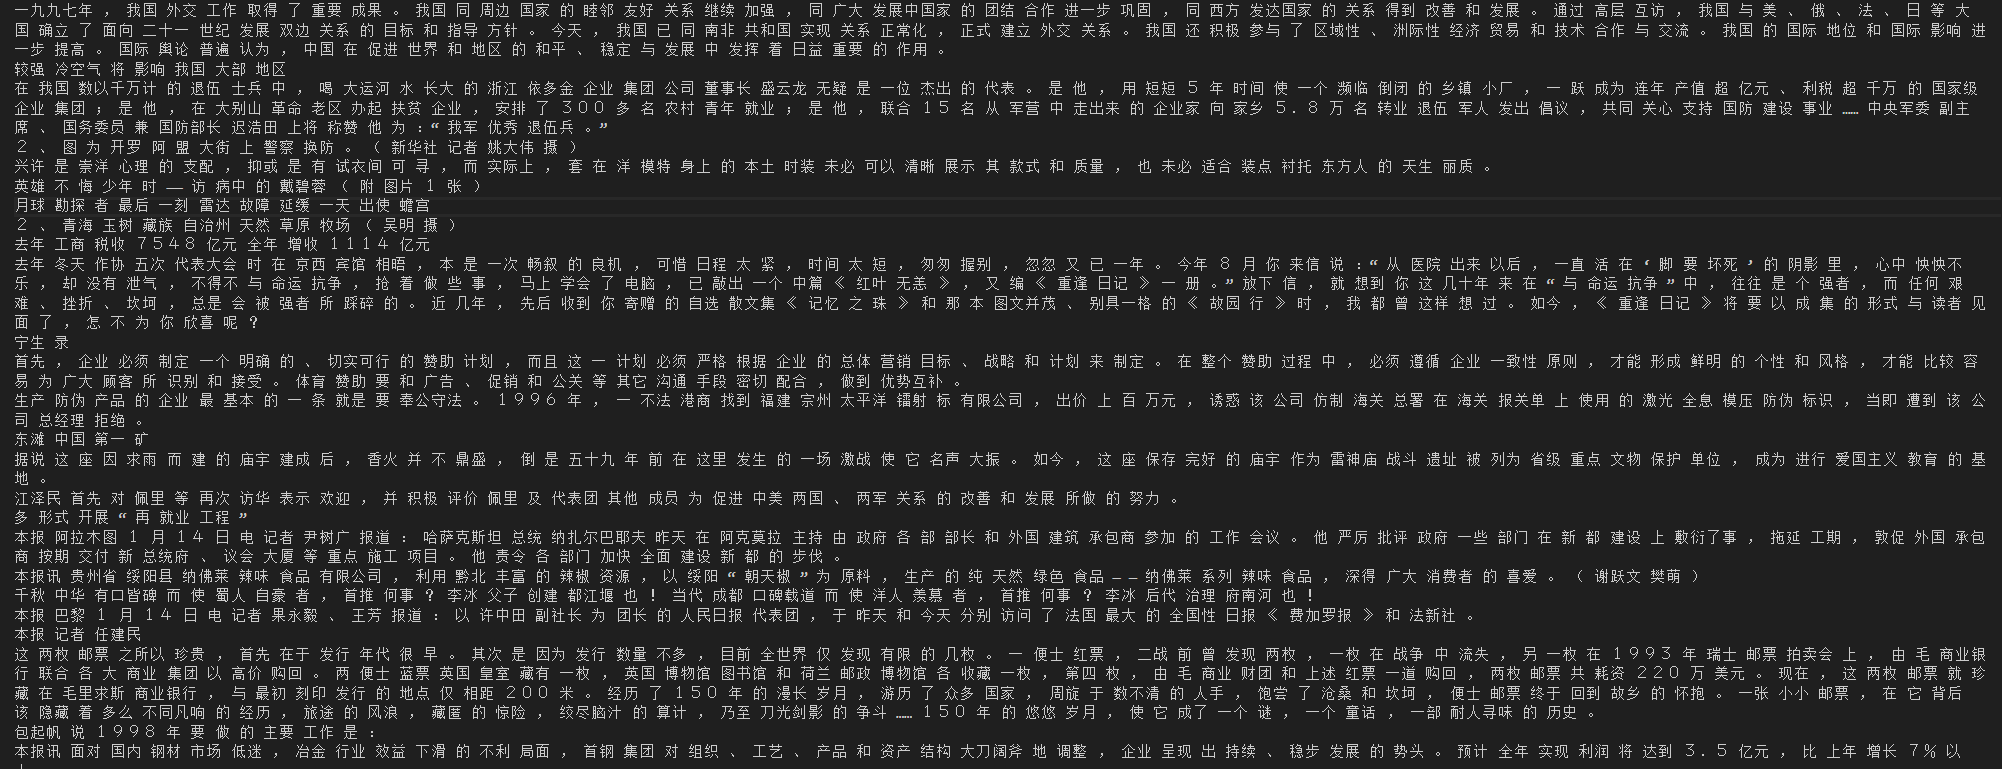
\includegraphics[width=0.8\textwidth]{image/2.png}
    \caption{DeepSeek-V3分词结果示例}
    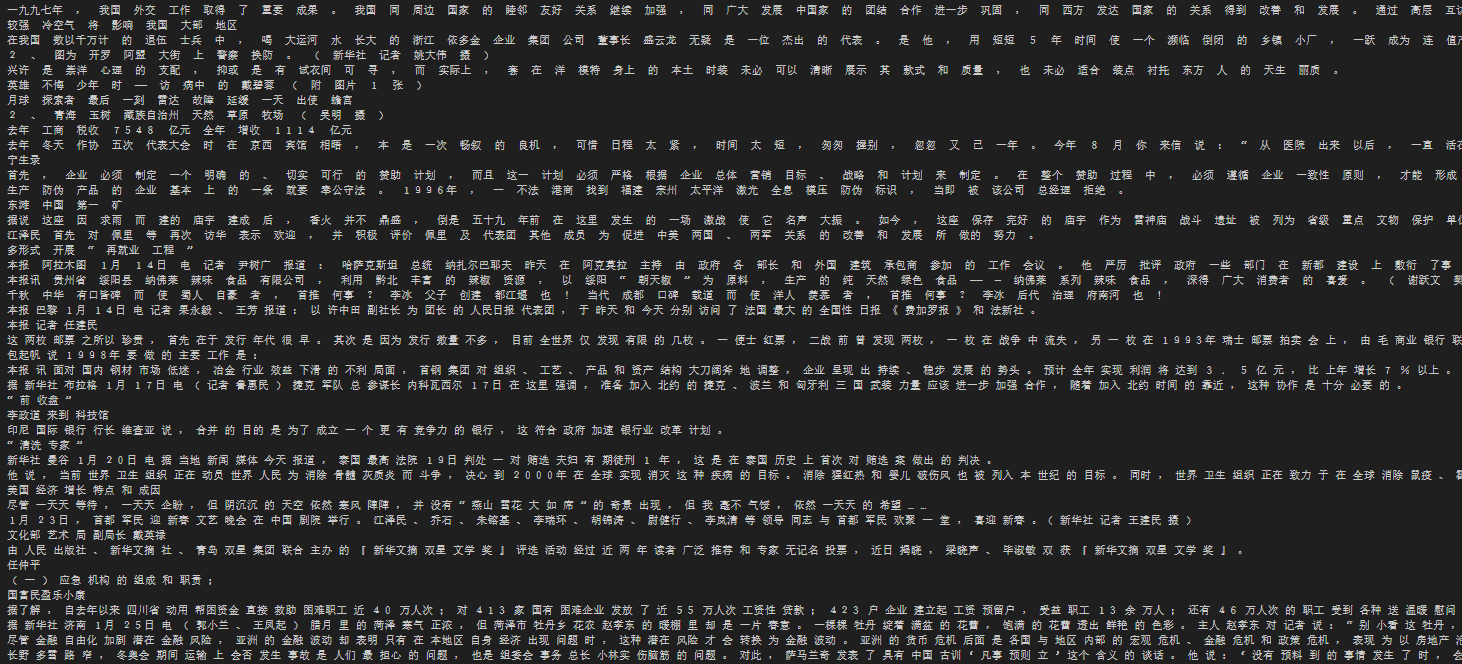
\includegraphics[width=0.8\textwidth]{image/4.png}
    \caption{Qwen3-8B分词结果示例}
    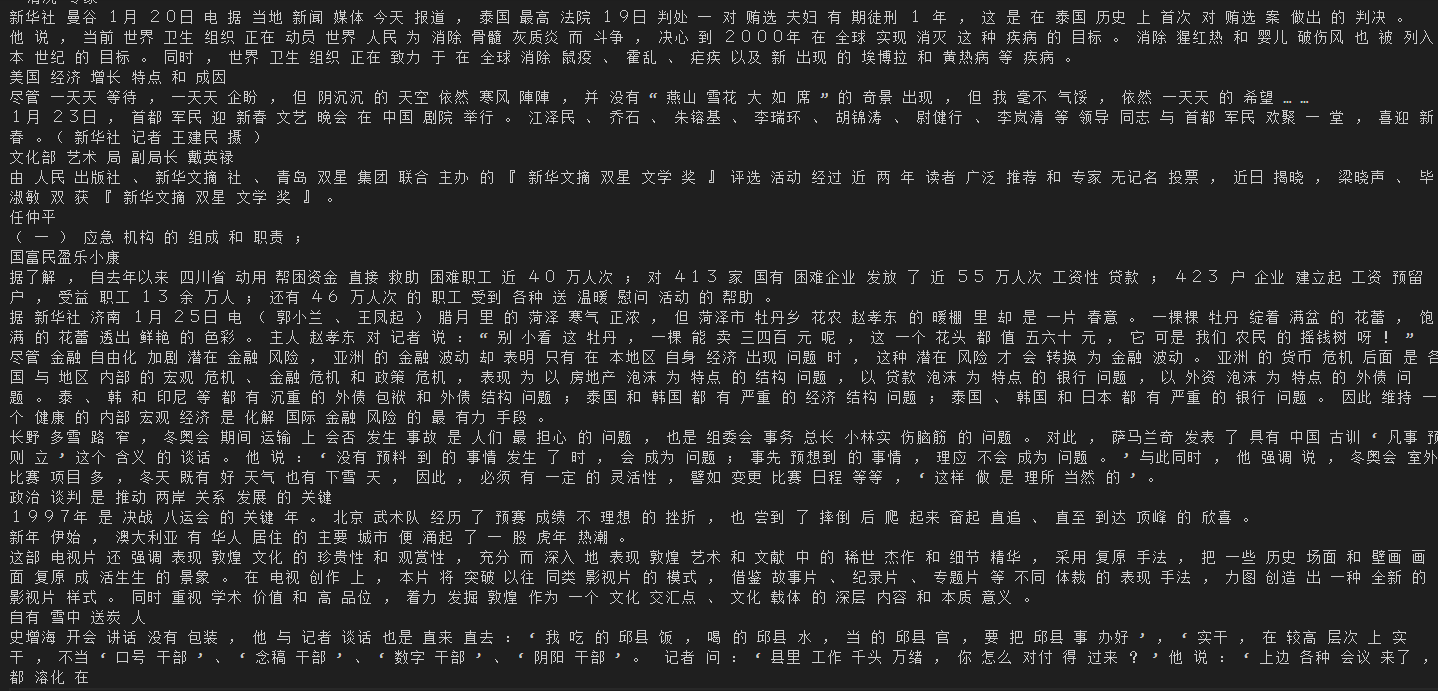
\includegraphics[width=0.8\textwidth]{image/3.png}
    \caption{Qwen3-32B分词结果示例}
    \label{fig:llm_example}
\end{figure}
值得注意的是，Qwen3-8B分词结果出现了不稳定结果即前20行的输出以两个空格为间隔分词，但在之后却变成了单个空格。在后面的任务中，Qwen3-8B仍然出现这种不稳定输出。
\subsection{实验结果}
表 \ref{tab:pku_result} 展示了三个模型在标准新闻语料上的表现。

\begin{table}[H]
    \centering
    \caption{各模型在《人民日报》测试集上的分词性能}
    \label{tab:pku_result}
    \begin{tabular}{l c c c}
        \toprule
        \textbf{Model} & \textbf{Precision (\%)} & \textbf{Recall (\%)} & \textbf{F1-Score (\%)} \\
        \midrule
        Qwen3-8B      & 79.00 & 74.42 & 76.65 \\
        Qwen3-32B     & 85.52& 84.54 & 85.03 \\
        DeepSeek-V3   & 88.55 & 86.84 & 87.69 \\
        \bottomrule
    \end{tabular}
\end{table}

\subsection{结果分析}
实验结果表明，大语言模型在零样本（Zero-shot）设置下的中文分词性能与其参数规模及模型架构呈现显著的正相关性。具体分析如下：

\begin{enumerate}
    \item \textbf{模型规模效应（Scaling Law）显著}：
    对比 Qwen3 系列的两个模型，Qwen3-32B 在 F1 值上达到了 85.03\%，相较于 Qwen3-8B 的 76.65\% 提升了约 8.38 个百分点。这表明随着参数量的增加，模型对长难句的语义理解能力和上下文依赖关系的捕捉能力显著增强，能够更准确地处理歧义切分问题。

    \item \textbf{顶级模型的性能优势}：
    DeepSeek-V3 取得了最优的实验结果（F1=87.69\%），在 Precision 和 Recall 上均全面领先。这主要归因于其更强的推理能力和在大规模中文语料上的充分预训练，使其在处理未登录词（OOV）和特定命名实体识别（NER）时表现更加稳健。

    \item \textbf{分词颗粒度偏好（Precision > Recall）}：
    观察所有模型的数据发现，准确率（Precision）普遍高于召回率（Recall）。这反映出通用大模型在分词风格上倾向于“粗颗粒度”（Coarse-grained）切分，即倾向于将“新世纪”、“大语言模型”等复合词视为一个整体，而《人民日报》（PKU）标准往往要求将其切分为更细的单元（如“新/世纪”）。这种标准不一致是导致 Recall 相对较低的主要原因。
\end{enumerate}

% --- 任务二 ---
\section{自采集文本分词能力测试}
\subsection{多源数据构建}
为了测试模型的泛化能力，利用 Python 爬虫获取了以下三类文本：
\begin{enumerate}
    \item \textbf{古诗文}：包含文言文和古汉语表达，句式较为复杂。
    \item \textbf{豆瓣评论}：口语化严重，且含有较多专业领域，如电影、图书相关词汇。
    \item \textbf{百度百科}：说明文性质，包含较多专有名词。
\end{enumerate}
\begin{figure}[H]
    \centering
    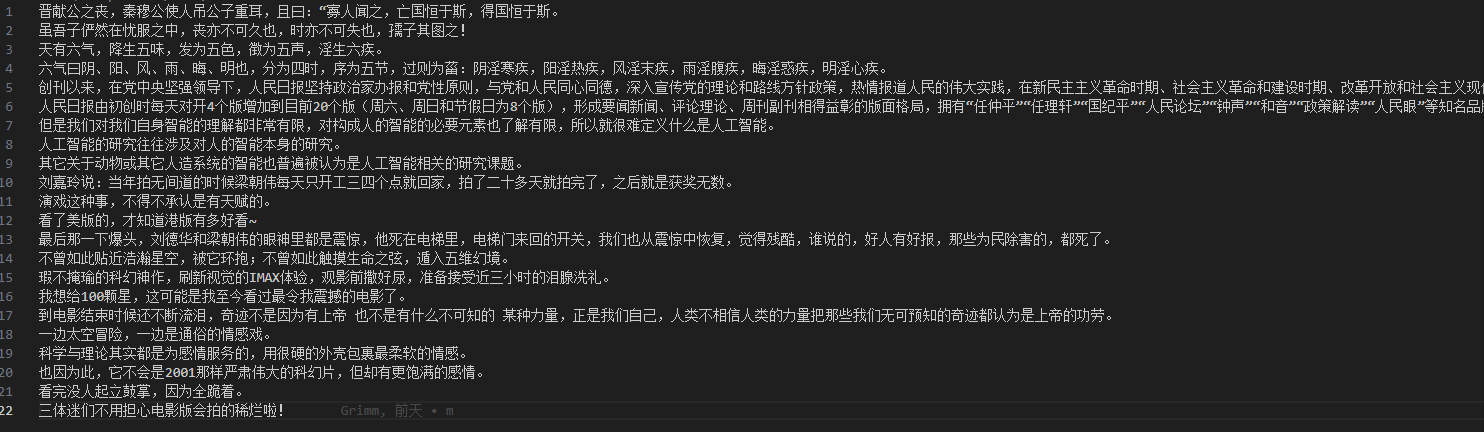
\includegraphics[width=0.8\textwidth]{image/5.png}
    \caption{多源文本示例}
    \label{fig:multi_source_example}
\end{figure}
\subsection{LLM分词结果}
以下为部分输出示例：
\begin{figure}[H]
    \centering
    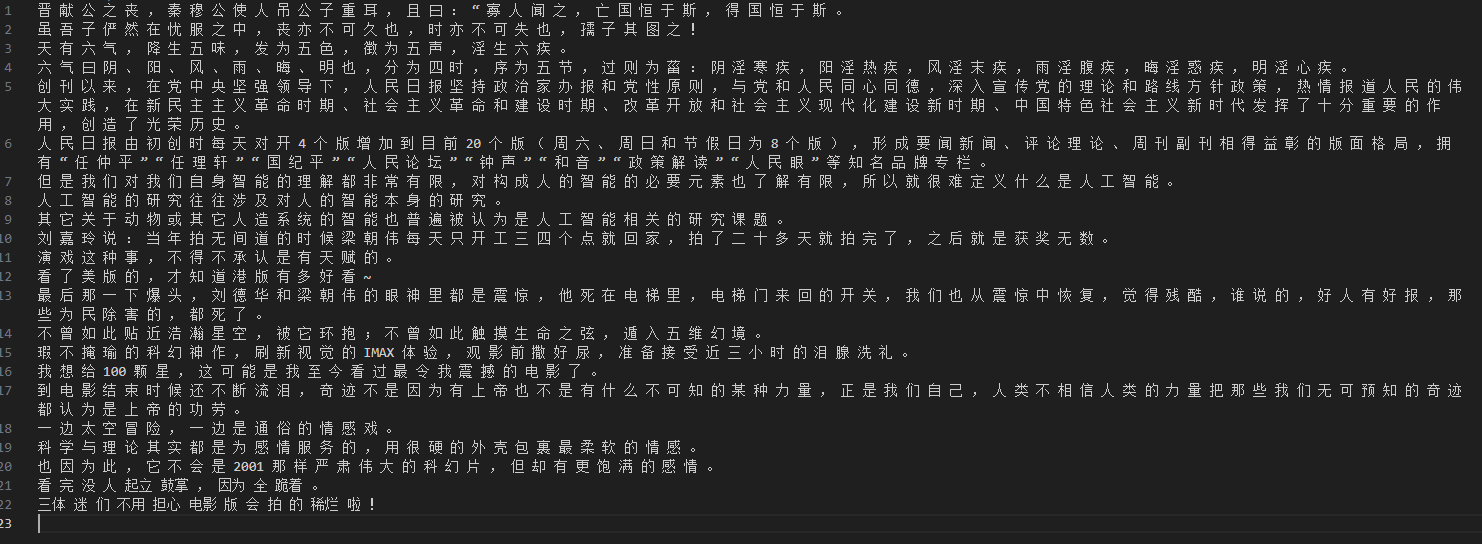
\includegraphics[width=0.8\textwidth]{image/6.png}
    \caption{DeepSeek-V3分词结果示例}
    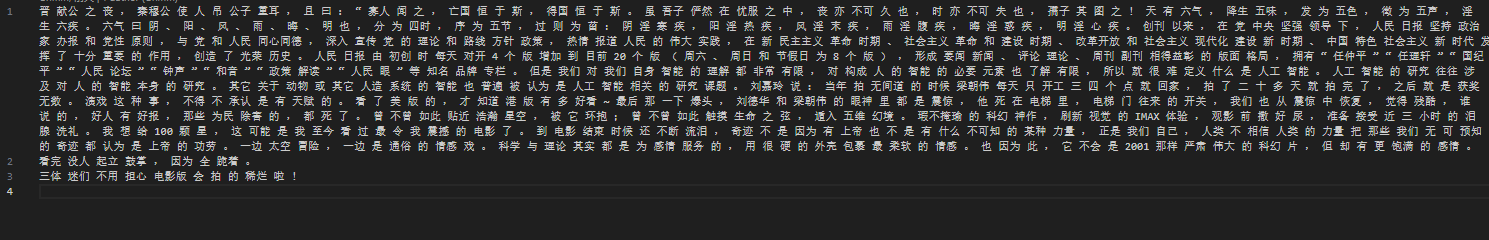
\includegraphics[width=0.8\textwidth]{image/7.png}
    \caption{Qwen3-8B分词结果示例}
    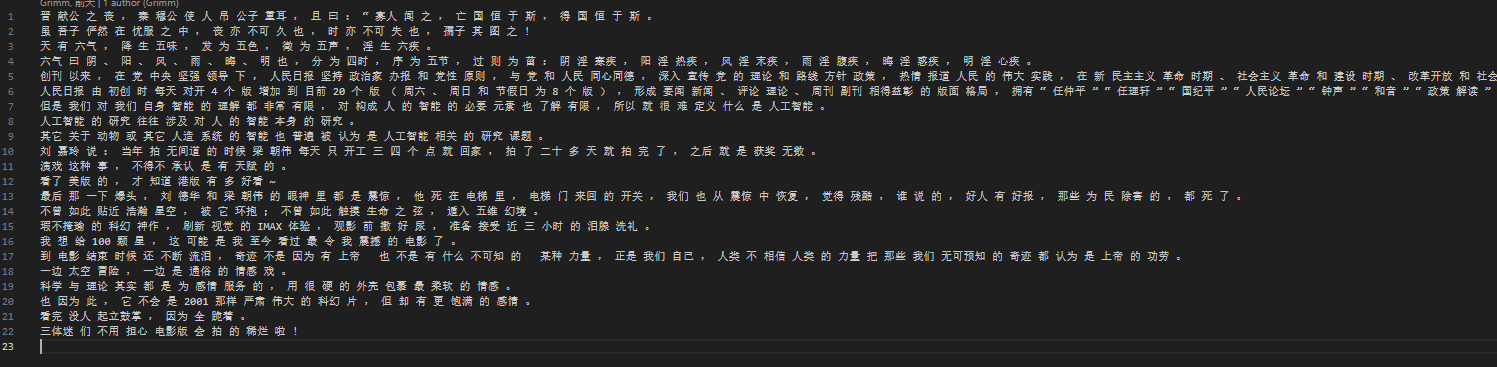
\includegraphics[width=0.8\textwidth]{image/8.png}
    \caption{Qwen3-32B分词结果示例}
    \label{fig:llm_multi_source_example}
\end{figure}

\subsection{实验结果与分析}
在本次实验中，不同模型的输出差异非常大。正如前文所说，Qwen3-8B的输出不稳定，在本次实验中，其输出甚至出现了错误分行。按照prompt的要求，模型应当保持输出的行数不变，但其却将部分行合并。此外，DeepSeek-V3分词结果只将最后两个例子分词正确，其余均未按照要求进行分词，只是将汉字一个一个隔开。因此对于无法给出量化结果的分析，仅给出定性分析。
\begin{table}[H]
    \centering
    \caption{Qwen32B在多源文本测试集上的分词性能}
    \label{tab:multi_source_result}
    \begin{tabular}{l c c c}
        \toprule
        \textbf{Model} & \textbf{Precision (\%)} & \textbf{Recall (\%)} & \textbf{F1-Score (\%)} \\
        \midrule
        Qwen3-32B     & 91.82& 87.76 & 89.74 \\
        DeepSeek-V3   & 44.17 & 62.54& 51.77 \\
        \bottomrule
    \end{tabular}
\end{table}
\begin{itemize}
    \item \textbf{Qwen3-32B表现优异}：在多源文本上，Qwen3-32B依然展现了强大的分词能力，取得了89.74\%的F1值，显示出其良好的泛化能力。模型能够较好地适应不同文本风格和领域的分词需求。
    \item \textbf{DeepSeek-V3和Qwen3-8B表现不佳}：DeepSeek-V3未能按照提示词要求进行分词，输出结果与预期差距较大，显示出其在处理多源文本时的局限性。Qwen3-8B则因输出不稳定，导致无法进行有效评估，反映出其在复杂文本处理上的不足。
 
\end{itemize}

\section{分词性能提升实验}
\subsection{优化方法：Few-Shot Prompting}
改进实验，我想验证基于 \textbf{Few-shot (In-Context Learning)} 的优化方法。

构造的 Prompt 包含 4 个典型示例，涵盖了人名、日期和成语的处理规范。
\begin{lstlisting}[language=Python]
FEW_SHOT_PROMPT = """
Below are some examples of standard Chinese Word Segmentation:

Example 1:
Input: 迈向充满希望的新世纪
Output: 迈向 充满 希望 的 新 世纪

Example 2:
Input: 中共中央总书记江泽民
Output: 中共中央 总书记 江泽民

Example 3:
Input: 1997年12月31日
Output: 1997年 12月 31日

Example 4:
Input: 提出并实验提升大模型在分词任务上性能的方法
Output: 提出 并 实验 提升 大 模型 在 分词 任务 上 性能 的 方法

Now, please segment the following lines strictly following the style above.
"""
\end{lstlisting}
\subsection{LLM分词结果}
以下为部分输出示例：
\begin{figure}[H]
    \centering
    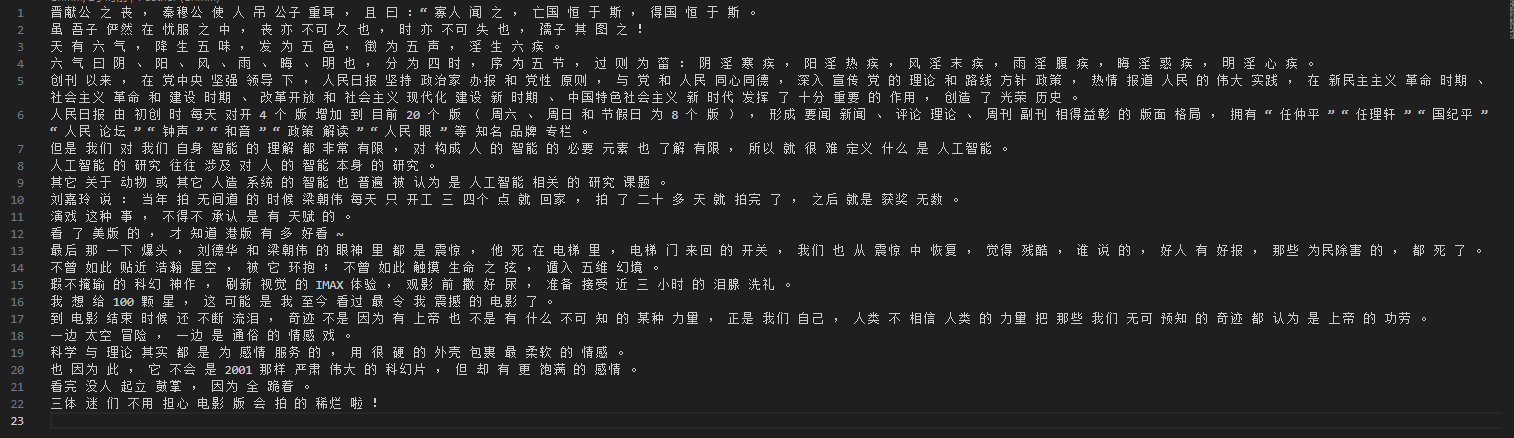
\includegraphics[width=0.8\textwidth]{image/9.png}
    \caption{DeepSeek-V3 Few-shot分词结果示例}
    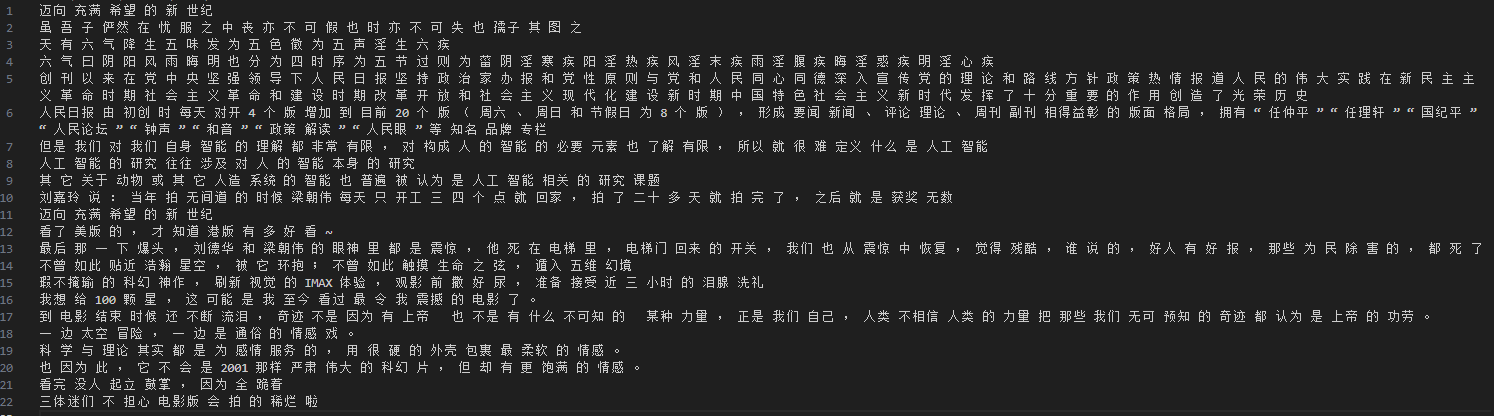
\includegraphics[width=0.8\textwidth]{image/10.png}
    \caption{Qwen3-8B Few-shot分词结果示例}
    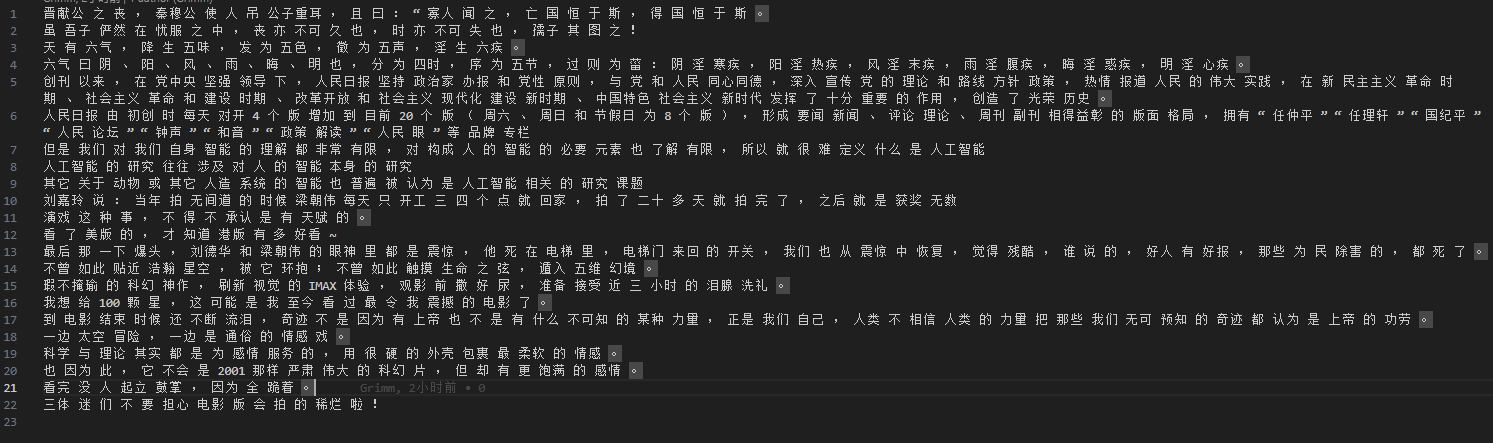
\includegraphics[width=0.8\textwidth]{image/11.png}
    \caption{Qwen3-32B Few-shot分词结果示例}
    \label{fig:few_shot_example}
\end{figure}
\subsection{实验结果与分析}
在引入 Few-shot 提示后，模型的分词性能均有显著提升。但是，Qwen3-8B 仍然存在输出不稳定的问题。DeepSeek-V3 和 Qwen3-32B 则均展现了强劲的分词能力。具体结果如下：
\begin{table}[H]
    \centering
    \caption{各模型在《人民日报》测试集上的Few-shot分词性能}
    \label{tab:few_shot_result}
    \begin{tabular}{l c c c}
        \toprule
        \textbf{Model} & \textbf{Precision (\%)} & \textbf{Recall (\%)} & \textbf{F1-Score (\%)} \\
        \midrule
        Qwen3-8B      & 72.47 & 70.65 & 71.55 \\
        Qwen3-32B     & 89.78 & 85.55 & 87.61 \\
        DeepSeek-V3   & 94.64 & 91.15 & 92.86 \\
        \bottomrule
    \end{tabular}
\end{table}
\section{结论}
本实验系统评估了大语言模型在中文分词任务上的表现。实验表明，参数量更大的模型具备更好的语言理解能力，且通过 Few-shot 提示工程可以显著纠正模型的分词风格，使其更贴近特定的标注规范（如 PKU 标准）。

\end{document}